\documentclass{standalone}
\usepackage{tikz}
\usetikzlibrary{arrows.meta,decorations.pathmorphing}

\begin{document}



\tikzset{every picture/.style={line width=0.75pt}} %set default line width to 0.75pt        

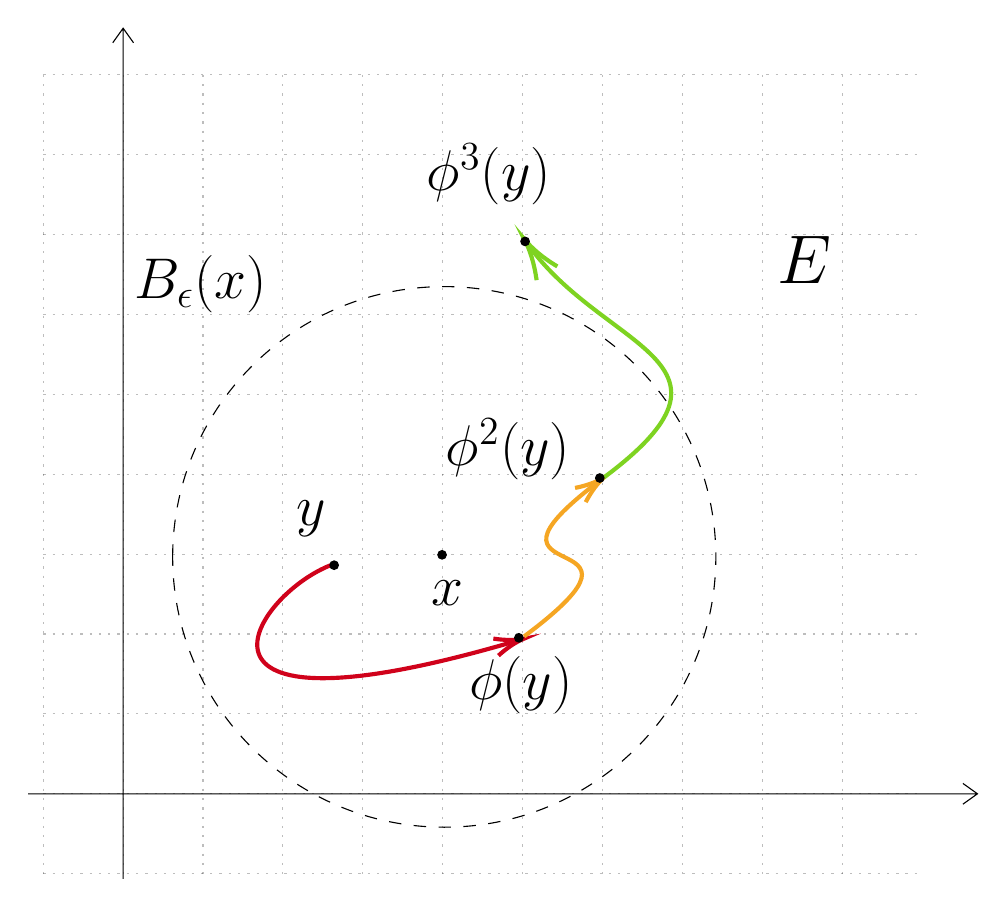
\begin{tikzpicture}[x=0.75pt,y=0.75pt,yscale=-1,xscale=1]
%uncomment if require: \path (0,446); %set diagram left start at 0, and has height of 446

%Shape: Axis 2D [id:dp5958965788842521] 
\draw  (26,374.85) -- (483.33,374.85)(71.73,6) -- (71.73,415.83) (476.33,369.85) -- (483.33,374.85) -- (476.33,379.85) (66.73,13) -- (71.73,6) -- (76.73,13)  ;
%Shape: Grid [id:dp9524606760405594] 
\draw  [draw opacity=0][dash pattern={on 0.84pt off 2.51pt}] (33.25,28.48) -- (456.59,28.48) -- (456.59,413.42) -- (33.25,413.42) -- cycle ; \draw  [color={rgb, 255:red, 0; green, 0; blue, 0 }  ,draw opacity=0.26 ][dash pattern={on 0.84pt off 2.51pt}] (33.25,28.48) -- (33.25,413.42)(71.73,28.48) -- (71.73,413.42)(110.22,28.48) -- (110.22,413.42)(148.7,28.48) -- (148.7,413.42)(187.19,28.48) -- (187.19,413.42)(225.67,28.48) -- (225.67,413.42)(264.16,28.48) -- (264.16,413.42)(302.64,28.48) -- (302.64,413.42)(341.13,28.48) -- (341.13,413.42)(379.62,28.48) -- (379.62,413.42)(418.1,28.48) -- (418.1,413.42) ; \draw  [color={rgb, 255:red, 0; green, 0; blue, 0 }  ,draw opacity=0.26 ][dash pattern={on 0.84pt off 2.51pt}] (33.25,28.48) -- (456.59,28.48)(33.25,66.97) -- (456.59,66.97)(33.25,105.45) -- (456.59,105.45)(33.25,143.94) -- (456.59,143.94)(33.25,182.42) -- (456.59,182.42)(33.25,220.91) -- (456.59,220.91)(33.25,259.39) -- (456.59,259.39)(33.25,297.88) -- (456.59,297.88)(33.25,336.36) -- (456.59,336.36)(33.25,374.85) -- (456.59,374.85)(33.25,413.34) -- (456.59,413.34) ; \draw  [color={rgb, 255:red, 0; green, 0; blue, 0 }  ,draw opacity=0.26 ][dash pattern={on 0.84pt off 2.51pt}]  ;
%Shape: Boxed Bezier Curve [id:dp8362135244366136] 
\draw [color={rgb, 255:red, 208; green, 2; blue, 27 }  ,draw opacity=1 ][line width=1.5]    (174.15,263.83) .. controls (135.76,276.46) and (83.9,353.69) .. (262.22,300.89) ;
\draw [shift={(264.93,300.09)}, rotate = 163.33] [color={rgb, 255:red, 208; green, 2; blue, 27 }  ,draw opacity=1 ][line width=1.5]    (14.21,-4.28) .. controls (9.04,-1.82) and (4.3,-0.39) .. (0,0) .. controls (4.3,0.39) and (9.04,1.82) .. (14.21,4.28)   ;
%Shape: Ellipse [id:dp48854496675935066] 
\draw  [dash pattern={on 4.5pt off 4.5pt}] (95.59,260.71) .. controls (95.59,188.79) and (154.18,130.48) .. (226.44,130.48) .. controls (298.71,130.48) and (357.29,188.79) .. (357.29,260.71) .. controls (357.29,332.63) and (298.71,390.94) .. (226.44,390.94) .. controls (154.18,390.94) and (95.59,332.63) .. (95.59,260.71) -- cycle ;
%Curve Lines [id:da41874514089187165] 
\draw [color={rgb, 255:red, 245; green, 166; blue, 35 }  ,draw opacity=1 ][line width=1.5]    (264.93,299.01) .. controls (341.13,242.13) and (228.73,279.1) .. (301.16,224.1) ;
\draw [shift={(303.41,222.41)}, rotate = 143.26] [color={rgb, 255:red, 245; green, 166; blue, 35 }  ,draw opacity=1 ][line width=1.5]    (14.21,-4.28) .. controls (9.04,-1.82) and (4.3,-0.39) .. (0,0) .. controls (4.3,0.39) and (9.04,1.82) .. (14.21,4.28)   ;
%Curve Lines [id:da39152174481105795] 
\draw [color={rgb, 255:red, 126; green, 211; blue, 33 }  ,draw opacity=1 ][line width=1.5]    (303.41,222.41) .. controls (379.23,165.82) and (302.89,161.25) .. (266.56,109.88) ;
\draw [shift={(264.93,107.5)}, rotate = 56.42] [color={rgb, 255:red, 126; green, 211; blue, 33 }  ,draw opacity=1 ][line width=1.5]    (19.89,-5.99) .. controls (12.65,-2.54) and (6.02,-0.55) .. (0,0) .. controls (6.02,0.55) and (12.65,2.54) .. (19.89,5.99)   ;
%Shape: Circle [id:dp7149274459952493] 
\draw  [fill={rgb, 255:red, 0; green, 0; blue, 0 }  ,fill opacity=1 ] (223.33,259.71) .. controls (223.33,258.57) and (224.25,257.65) .. (225.39,257.65) .. controls (226.52,257.65) and (227.44,258.57) .. (227.44,259.71) .. controls (227.44,260.84) and (226.52,261.76) .. (225.39,261.76) .. controls (224.25,261.76) and (223.33,260.84) .. (223.33,259.71) -- cycle ;
%Shape: Circle [id:dp7171311598003665] 
\draw  [fill={rgb, 255:red, 0; green, 0; blue, 0 }  ,fill opacity=1 ] (171.33,264.71) .. controls (171.33,263.57) and (172.25,262.65) .. (173.39,262.65) .. controls (174.52,262.65) and (175.44,263.57) .. (175.44,264.71) .. controls (175.44,265.84) and (174.52,266.76) .. (173.39,266.76) .. controls (172.25,266.76) and (171.33,265.84) .. (171.33,264.71) -- cycle ;
%Shape: Circle [id:dp2525359311831692] 
\draw  [fill={rgb, 255:red, 0; green, 0; blue, 0 }  ,fill opacity=1 ] (260.33,299.71) .. controls (260.33,298.57) and (261.25,297.65) .. (262.39,297.65) .. controls (263.52,297.65) and (264.44,298.57) .. (264.44,299.71) .. controls (264.44,300.84) and (263.52,301.76) .. (262.39,301.76) .. controls (261.25,301.76) and (260.33,300.84) .. (260.33,299.71) -- cycle ;
%Shape: Circle [id:dp19254067806539155] 
\draw  [fill={rgb, 255:red, 0; green, 0; blue, 0 }  ,fill opacity=1 ] (299.33,222.71) .. controls (299.33,221.57) and (300.25,220.65) .. (301.39,220.65) .. controls (302.52,220.65) and (303.44,221.57) .. (303.44,222.71) .. controls (303.44,223.84) and (302.52,224.76) .. (301.39,224.76) .. controls (300.25,224.76) and (299.33,223.84) .. (299.33,222.71) -- cycle ;
%Shape: Circle [id:dp22569853940877072] 
\draw  [fill={rgb, 255:red, 0; green, 0; blue, 0 }  ,fill opacity=1 ] (263.33,108.71) .. controls (263.33,107.57) and (264.25,106.65) .. (265.39,106.65) .. controls (266.52,106.65) and (267.44,107.57) .. (267.44,108.71) .. controls (267.44,109.84) and (266.52,110.76) .. (265.39,110.76) .. controls (264.25,110.76) and (263.33,109.84) .. (263.33,108.71) -- cycle ;

% Text Node
\draw (218.84,270.87) node [anchor=north west][inner sep=0.75pt]  [font=\huge]  {$x$};
% Text Node
\draw (385.58,104.93) node [anchor=north west][inner sep=0.75pt]  [font=\Huge]  {$E$};
% Text Node
\draw (237.16,307.28) node [anchor=north west][inner sep=0.75pt]  [font=\huge]  {$\phi (y)$};
% Text Node
\draw (225.99,192.79) node [anchor=north west][inner sep=0.75pt]  [font=\huge]  {$\phi ^{2}(y)$};
% Text Node
\draw (216.76,60.63) node [anchor=north west][inner sep=0.75pt]  [font=\huge]  {$\phi ^{3}(y)$};
% Text Node
\draw (75.91,114.31) node [anchor=north west][inner sep=0.75pt]  [font=\huge]  {$B_{\epsilon }( x)$};
% Text Node
\draw (154,232.4) node [anchor=north west][inner sep=0.75pt]  [font=\huge]  {$y$};


\end{tikzpicture}
\end{document}